\documentclass[conference]{IEEEtran}
\IEEEoverridecommandlockouts
% The preceding line is only needed to identify funding in the first footnote. If that is unneeded, please comment it out.
\usepackage{cite}
\usepackage{amsmath,amssymb,amsfonts}
\usepackage{algorithmic}
\usepackage{graphicx}
\usepackage{textcomp}
\usepackage{xcolor}
\usepackage{hyperref}
\usepackage[ngerman]{babel}

\def\BibTeX{{\rm B\kern-.05em{\sc i\kern-.025em b}\kern-.08em
    T\kern-.1667em\lower.7ex\hbox{E}\kern-.125emX}}
\begin{document}

\title{Augmented Reality in Education
}

\author{\IEEEauthorblockN{Tobias Wen Klingenberg}
\IEEEauthorblockA{\textit{School of Computation, Information and Technology} \\
\textit{Technische Universität München}\\
München, Deutschland \\
t.klingenberg@tum.de}
}
\maketitle

\begin{abstract}
Innovation in der Bildung ist seit jeher eine erstrebenswerte, aber meißt nicht
vorhandene oder durchsetzbare Thematik die in den letzten Jahren immer mehr 
Aufmerksamkeit bekommen hat. Eine dieser Innovationen ist die Augmented Reality
(Erweiterte Realität), welche tatsächlich sehr sinnvolle und bereichernde 
Möglichekiten für die Bildung bieten kann.
Das folgende Paper befasst sich mit der Entwicklung, 
Anwendung und Analyse der Möglichkeiten von Augmented Reality 
in der Bildung.
\end{abstract}

\section{Einleitung}
Augmented Reality (im Folgenden AR) ist eine Innovation, welche in den letzten
Jahren immer mehr Akzeptanz und tatsächliche Anwendung in unserem täglichen
Leben genießen konnte. Sie ist eine Technologie, welche es ermöglicht, digitale
Informationen mit der echten physischen Welt zu überlagern und somit die persönliche 
Sicht ''erweitern''.

Dazu gibt es verschiedenste Innovationen, die dieses Konzept 
auf unterschiedlicher Weise ermöglichen. Durch diese Verschmelzung
der digitalen und realen Welt eröffnen sich vollkommen neue Anwendungsmöglichkeiten
, wie unter anderem interaktive Lernumgebungen, Unterstützung im medizinischen Bereich
oder Unterhaltungs- und Unterstützungsmedien. Im Folgenden wird vor allem auf die möglichen 
Anwendungen im Bildungsbereich eingegangen.


\section{Warum AR}

AR bietet sich vor allem aus mehreren Gründen für eine Anwendung in den verschiedensten
Bildungsmöglichkeiten an. Dazu gehört vor allem eine stärkere Gedächtnisleistung aufgrund von
visuellen und interaktiven Inhalten, sowie ein personalisiertes Lernen durch Anpassung 
auf individuell nötigen Bedürfnissen \cite{b1}. 

Eine hohe Motivation unter den Schüler:innen 
kann mit Ansätzen einer spielerischen Bildung ermöglicht werden. Vor allem interssant ist 
die mögliche kontextualisierte Lernerfahrung, indem theoretisches Wissen in simulierten 
Umgebungen angewedent werden kann \cite{b2}. TODO

\section{Entwicklung}
In den vergangen Jahren ließ sich eine immer höhrer Nachfrage für AR Technologien im Bildungsbereich
feststellen. Vor allem in der Forschung ist dieser Trend sichtbar, in der tatsächlichen Anwendung ist die
Adaption von diesen Technologien zwar vorhanden, jedoch noch immer nicht weitverbreitet \cite{b3}.

In \ref{fig1} lässt sich die Entwicklung des Themas Bildung mit AR darstellen. Die Abbildung zeigt die Anzahl
der veröffentlichten Paper in diesem Bereich von 2014 bis 2020 \cite{w2}. Ein klarer Sprung lässt sich in dem Jahr 2014 feststellen,
in welchem die Google Glasses vorgestellt wurden. Diese ermöglichten eine tatsächliche konsumentenorientiertete 
Möglichkeit, AR selbst umzusetzen. Dadurch wurde die Forschungsintensität in diesem Bereich verstärkt. 
Ein ähnlicher Sprung lässt sich im Jahr 2020 erkennen, welcher wohlmöglich aufgrund der Covid-19 Pandemie einen
Forschungsschwerpunkt in Richtung von Remote Unterricht als Grund hat.

\begin{figure}[htbp]
    \centerline{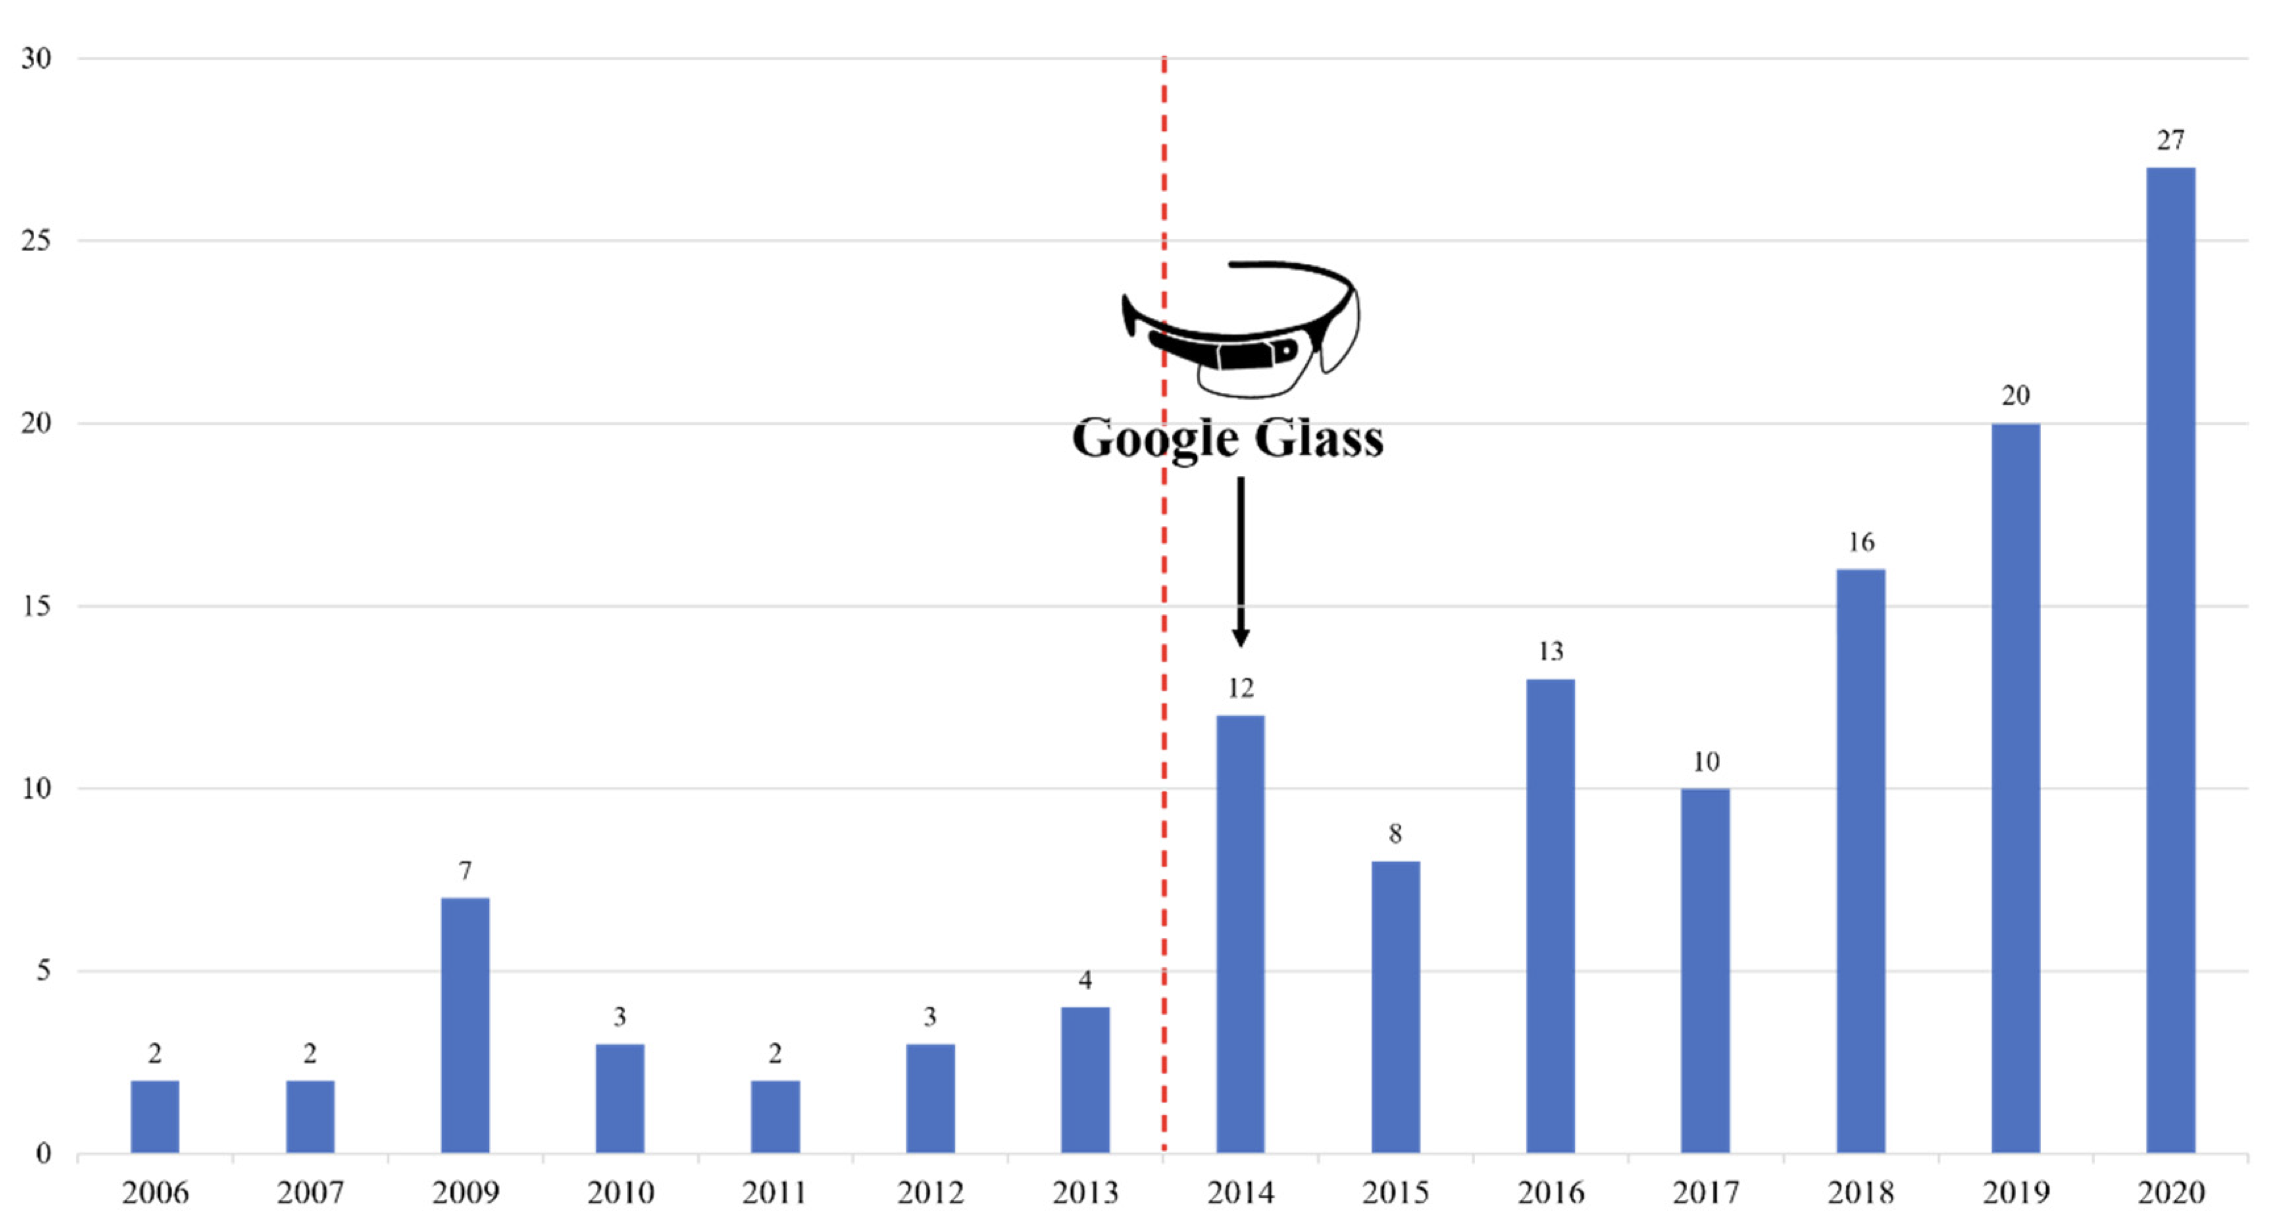
\includegraphics[scale=0.2]{img/entwicklung.png}}
    \caption{Anzahl an Paper über AR in der Bildung}
    \label{fig1}
\end{figure}

\section{AR-Tools und Plattformen}\label{AA}
Damit AR in der Bildung funktionieren kann, müssen einige Kriterien erfüllt sein. Das Zusammenspiel
zwischen Software und Hardware ist essenziel um eine immersive und interaktive Lernerfahrung
zu ermöglichen. Moderne Software ermöglicht es, Laborexperimente oder geschichtliche Ausflüge
zu veranstalten. Damit dies nahtlos in den Unterricht integriert werden kann, ist es wichtig, passende
Hardware zu unterstützen.
Im folgenden werden auf diese eingegangen und an einigen realen Beispielen diskutiert.

\subsection{Software}
Damit die Software in den Bildungssektor passt, müssen Kriterien wie eine einfache Bedienung,
weite Verbreitung, kostengünstig und passenden Inhalt gewährleistet sein. Momentan
vorhandene Beispiele sind unter anderem:
\begin{itemize}
    \item \href{https://sites.google.com/dublinschools.net/vr-ar/google-geo-tools/google-expeditions}{Google Expeditions}
    \item \href{https://koerber-stiftung.de/projekte/eustory/teaching-and-learning-in-the-metaverse/}{Metaverse}
    \item \href{https://www.4danatomy.com/}{Anatomy 4D}
    \item \href{https://www.labster.com/}{Labster}
    \item \href{https://www.cospaces.io/}{CoSpaces Edu}
\end{itemize}
Jedes dieser Beispiele fokussiert isch auf einen speziellen Fachbereich
in der Bildung. Während Google Expeditions sich auf virtuelle sowie augmentierte
Erlebnisse und Ausflüge fokussiert, passt sich unter anderem Anatomy 4D speziell
auf die Lehre der Biologie im Bereich Anatomie von Mensch und Tier ab. 
Labster ermöglicht es, teilweise Laborumgebungen zu augmentieren und so völlig neue
Lernumgebungen zu schaffen. Mithilfe von CoSpaces Edu lässt sich unter anderem
das Zusammenarbeiten trotz Distanz ermöglichen, indem andere Personen und Räume in 
den eigenen augmentiert werden können. \cite{w1}

\subsection{Hardware}
Damit die Hardware in den Bereich Bildung passt, muss auf einige Kriterien geachtet werden.
Unter anderem sollte, vor allem in der Benutzung im primären Bildungssektor, auf eine günstige
Hardwareoption geachtet werden. Diese sollte einfach zu bedienen sein und nich zu zerbrechlich sein.
In der Schule sind für diese Anwendung vor allem bereits vorhandene Hardware zu betrachten, zum Beispiel
LiDAR fähige Tablets sowie Smartphones und Computer die im Sinne der Schule bereits in das Curriculum
integriert sind. Diese benötigen teils keine weiteren Anschaffungskosten und auch keine weitere Schulung und
Weiterbildung der Lehrkräfte und Schüler.

Im Hinblick auf Bildung in der Hochschule und Weiterbildung in der Industrie sind vor allem kostenintesivere,
aber auch immersivere Hardwareoptionen möglich. Darunter gehöhren AR-Brillen und Headsets im Sinne von HUP (Head-up-Display),
Optical see through und Visual see through. Desweiteren gibt es speziell auf Bildung angepasste Hardware wie der 
\href{https://mergeedu.com/cube?cr=4646}{Merge Cube}, welcher es ermöglicht Schülern 3 dimensionale Objekte in der Hand zu
halten und damit zu interagieren. \href{https://zspace.com/}{ZSpace} hingegen ermöglicht es, dem Anwender mithilfe eines Stylus 
ähnlichen Stiftes, Objekte aus dem Monitor zu ziehen und dieses zu manipulieren.

Zu den wichtigsten Beispielen gehören unter anderem:
\begin{itemize}
    \item \href{https://www.microsoft.com/de-de/hololens}{Microsoft HoloLens}
    \item \href{https://www.meta.com/de/quest/quest-3/}{Meta Quest 3}
    \item \href{https://www.apple.com/de/apple-vision-pro/}{Apple Vision Pro}
\end{itemize}

Während das Microsoft HoloLens auf Optical see through setzt, benutzen beide anderen Beispiel Video see through, durch welche
zwar immersivere Erlebnisse gestaltbar sind, jedoch auch Nachteile durch Übelkeit möglich sind.


\section{Virtuelle Räume}
Gerade seit der Covid-19 Pandemie ist auch das Theme der virtuellen Klassenräume interessant geworden.
Dabei ist zu Unterscheiden zwischen dem virtuelle Klassenraum vor Ort und dem von anderen Orten aus.
Das Konzept besteht darin, dass entweder der Klassenraum an sich durch AR erweitert wird und somit der Unterricht
immersiv berreichert wird und, dass der Klassenraum vollkommen in einen anderen Raum augmentiert wird und somit
ein authentischer Unterricht von anderen Orten möglich ist.

\subsection{vor Ort}


\subsection{Remote}

\section{Anwendungen}
\textbf{The class file is designed for, but not limited to, six authors.} A 
minimum of one author is required for all conference articles. Author names 
should be listed starting from left to right and then moving down to the 
next line. This is the author sequence that will be used in future citations 
and by indexing services. Names should not be listed in columns nor group by 
affiliation. Please keep your affiliations as succinct as possible (for 
example, do not differentiate among departments of the same organization).

\subsection{Primär und Sekundär}
Headings, or heads, are organizational devices that guide the reader through 
your paper. There are two types: component heads and text heads.

Component heads identify the different components of your paper and are not 
topically subordinate to each other. Examples include Acknowledgments and 
References and, for these, the correct style to use is ``Heading 5''. Use 
``figure caption'' for your Figure captions, and ``table head'' for your 
table title. Run-in heads, such as ``Abstract'', will require you to apply a 
style (in this case, italic) in addition to the style provided by the drop 
down menu to differentiate the head from the text.

Text heads organize the topics on a relational, hierarchical basis. For 
example, the paper title is the primary text head because all subsequent 
material relates and elaborates on this one topic. If there are two or more 
sub-topics, the next level head (uppercase Roman numerals) should be used 
and, conversely, if there are not at least two sub-topics, then no subheads 
should be introduced.

\subsection{Hochschule}
Place figures and tables at the top and 
bottom of columns. Avoid placing them in the middle of columns. Large 
figures and tables may span across both columns. Figure captions should be 
below the figures; table heads should appear above the tables. Insert 
figures and tables after they are cited in the text. Use the abbreviation 
``Fig.~\ref{fig}'', even at the beginning of a sentence.


\begin{figure}[htbp]
\centerline{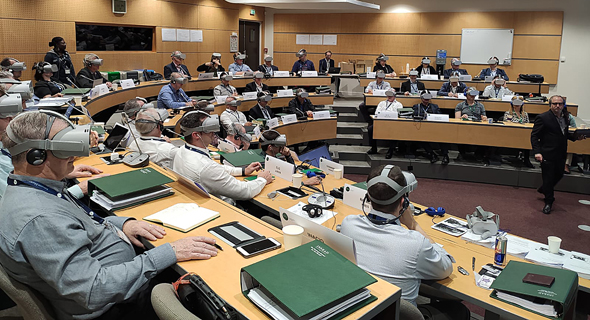
\includegraphics[scale=0.4]{img/fig2.jpg}}
\caption{Example of a figure caption.}
\label{fig}
\end{figure}

Figure Labels: Use 8 point Times New Roman for Figure labels. Use words 
rather than symbols or abbreviations when writing Figure axis labels to 
avoid confusing the reader. As an example, write the quantity 
``Magnetization'', or ``Magnetization, M'', not just ``M''. If including 
units in the label, present them within parentheses. Do not label axes only 
with units. In the example, write ``Magnetization (A/m)'' or ``Magnetization 
\{A[m(1)]\}'', not just ``A/m''. Do not label axes with a ratio of 
quantities and units. For example, write ``Temperature (K)'', not 
``Temperature/K''.

\section{Weiterbildung}

The preferred spelling of the word ``acknowledgment'' in America is without 
an ``e'' after the ``g''. Avoid the stilted expression ``one of us (R. B. 
G.) thanks $\ldots$''. Instead, try ``R. B. G. thanks$\ldots$''. Put sponsor 
acknowledgments in the unnumbered footnote on the first page.

\section{Potential}

Please number citations consecutively within brackets \cite{b1}. The 
sentence punctuation follows the bracket \cite{b2}. Refer simply to the reference 
number, as in \cite{b3}---do not use ``Ref. \cite{b3}'' or ``reference \cite{b3}'' except at 
the beginning of a sentence: ``Reference \cite{b3} was the first $\ldots$''

Number footnotes separately in superscripts. Place the actual footnote at 
the bottom of the column in which it was cited. Do not put footnotes in the 
abstract or reference list. Use letters for table footnotes.

Unless there are six authors or more give all authors' names; do not use 
``et al.''. Papers that have not been published, even if they have been 
submitted for publication, should be cited as ``unpublished'' \cite{b4}. Papers 
that have been accepted for publication should be cited as ``in press'' \cite{b5}. 
Capitalize only the first word in a paper title, except for proper nouns and 
element symbols.

For papers published in translation journals, please give the English 
citation first, followed by the original foreign-language citation \cite{b6}.

\begin{thebibliography}{00}
\bibitem{b1}  Dunleavy, M., Dede, C., and Mitchell, R. "Affordances and Limitations of Immersive Participatory Augmented Reality Simulations for Teaching and Learning". Journal of Science Education and Technology, 2009.
\bibitem{b2} Santos, M. E. C., Chen, A., Taketomi, T., Yamamoto, G., Miyazaki, J., and Kato, H, "Augmented Reality Learning Experiences: Survey of Prototype
Design and Evaluation". IEEE Transactions on Learning Technologies, 2014.
\bibitem{b3} Bacca, J., Baldiris, S., Fabregat, R., Graf, S., and Kinshuk, "Augmented Reality Trends in Education: A Systematic Review of Research and Applications". Educational Technology and Society, 2014.
\bibitem{b4} J. Zhang, G. Li, Q. Huang, Q. Feng and H. Luo, „Augmented Reality in K–12 Education A Systematic Review and Meta-Analysis of the Literature from 2000 to 2020”, MDPI, 2022.
\bibitem{b5} Akçayır, M., and Akçayır, G., "Advantages and challenges associated with augmented reality for education: A systematic review of the literature". Educational Research Review, 2017.
\bibitem{b6} Chen, P., Liu, X., Cheng, W., and Huang, R. ,"A review of using augmented reality in education from 2011 to 2016". Innovations in Smart Learning, 2017.
\bibitem[W1]{w1} \href{https://www.cospaces.io/tech-check-ar-with-smartphones}{https://www.cospaces.io/tech-check-ar-with-smartphones} letzter Zugriff 07.07.2024 16:32
\bibitem[W2]{w2} \href{https://www.marketresearchfuture.com/reports/ar-vr-in-education-market-10834}{https://www.marketresearchfuture.com/reports/ar-vr-in-education-market-10834} letzter Zugriff 03.07.2024 20:38
\end{thebibliography}
\vspace{12pt}

\end{document}
